\chapter{Implementation}


\newcommand*{\runner}{\textit{Runner}}
\newcommand*{\synthesizer}{\textit{Synthesizer}}
\newcommand*{\approximators}{\textit{Approximator}}
\newcommand*{\optimizer}{\textit{Optimizer}}

\label{sec:implementation}
{\name} is implemented in Python. It has four main components: {\runner}, {\synthesizer}, {\approximators}, and {\optimizer}. The relationships of four components are shown in Figure~\ref{fig:overview}. 
 

\begin{figure}[t]
    \centering
    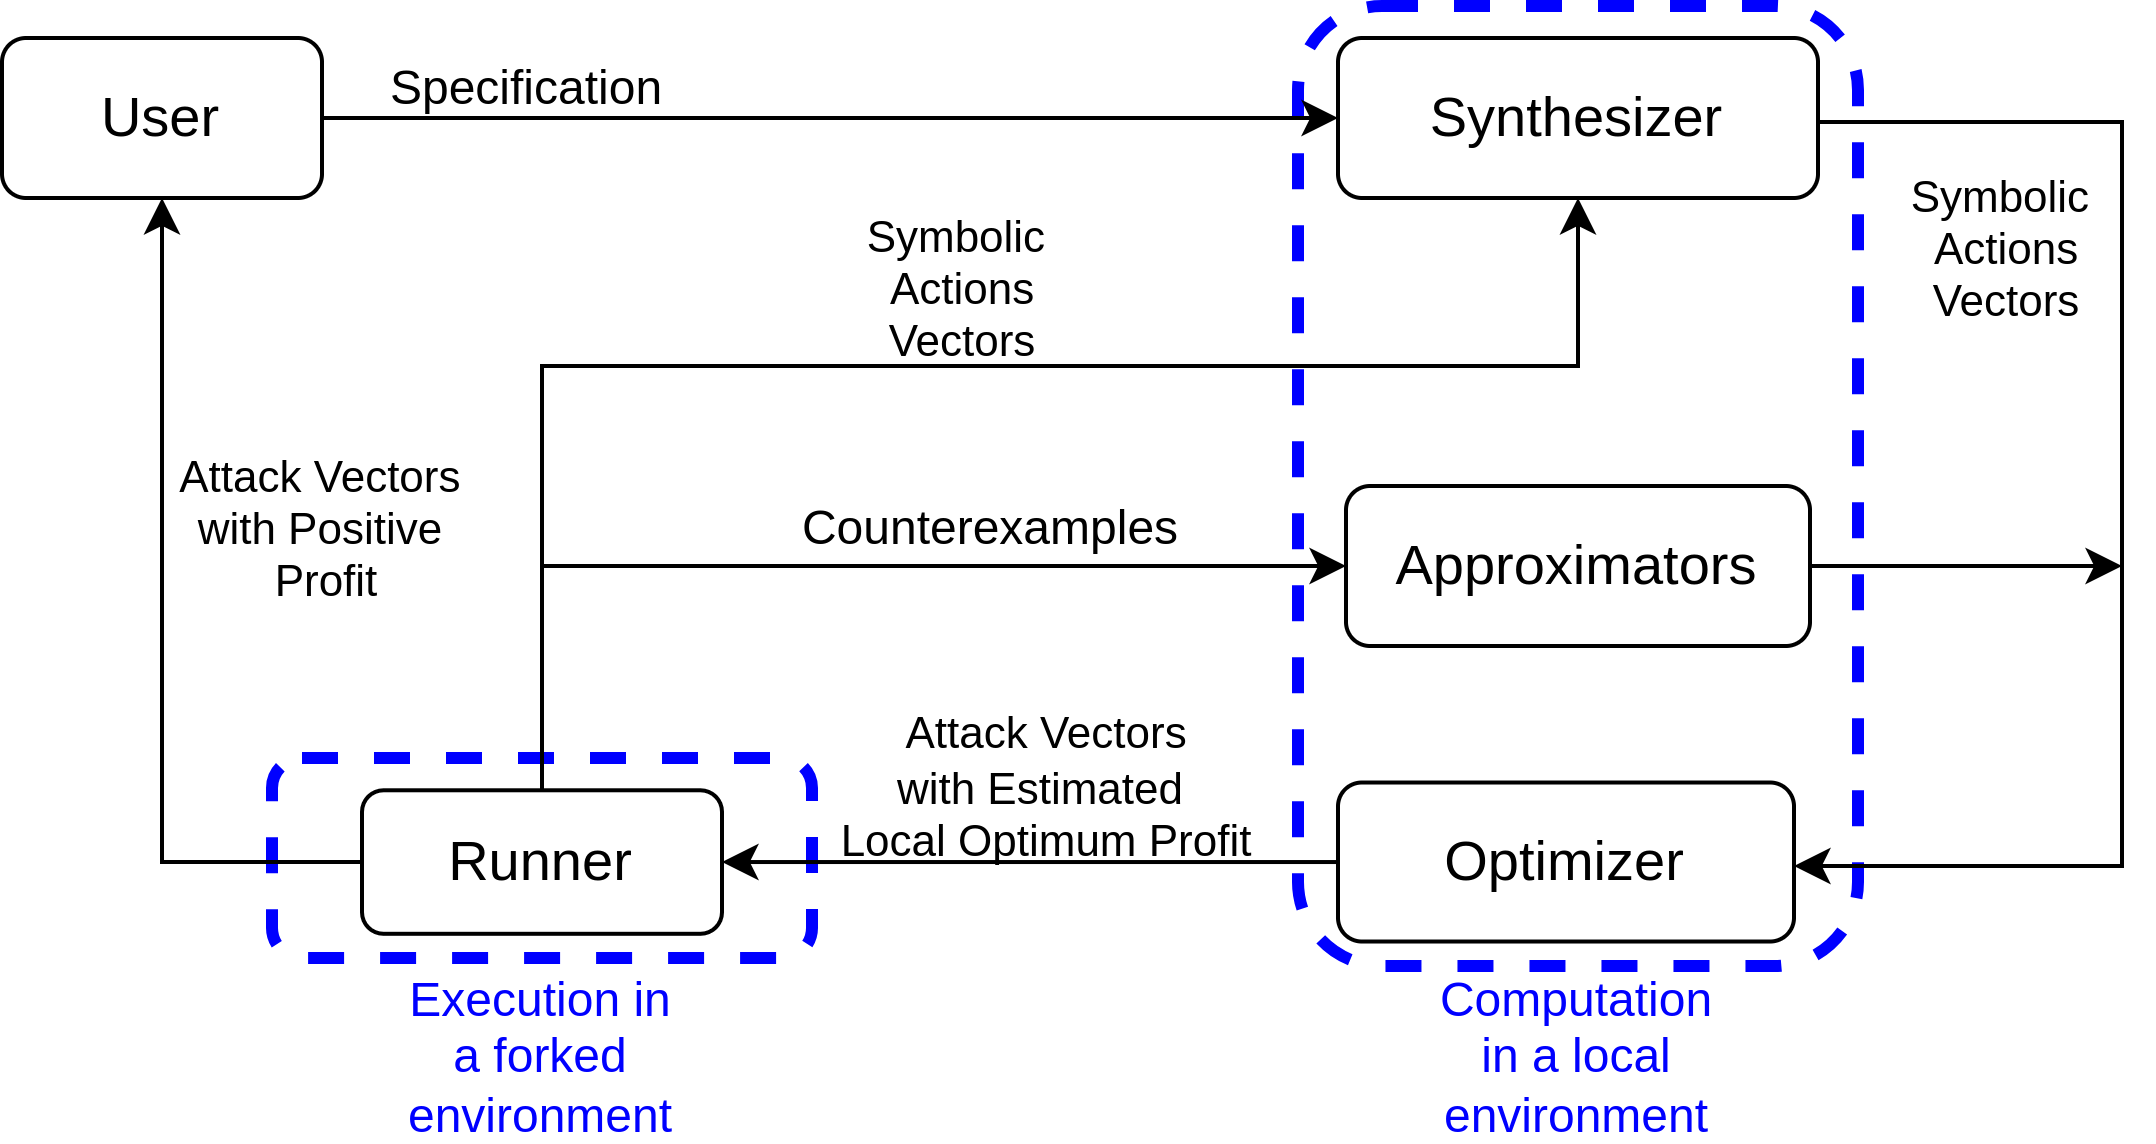
\includegraphics[width=\linewidth]{figures/overview2.png}
    \caption{The overview of our implementation}
    \label{fig:overview}
\end{figure}


\section{Overview}
{\name} takes as inputs a blockchain specification, initial flash loan amounts and a set actions with their specifications. %-(prestates, poststates, input tokens, output tokens). 
The {\runner} is responsible for the simulated environment based on a forked blockchain client. It performs both initial and counterexample based data collection. {\runner} is also used to check whether a candidate attack vector can really yield the estimated positive profit. These data points are used to construct {\approximators}, approximations to actions' transition functions.%(not shown in Figure~\ref{fig:overview}). 
The {\synthesizer} component prunes and enumerates actions vectors based on action specifications. 
The {\approximators} is responsible for the transition functions approximation using data points collected by the {\runner}. Finally, the {\optimizer} builds an optimization problem based on the approximated transition functions returned by {\approximators} for each symbolic actions vector enumerated by {\synthesizer} and performs global optimization on it. The obtained attack vector that yields a positive profit is executed by {\runner} to confirm the accuracy of the estimation. If the estimation is inaccurate the attack vector is treated as a counterexample and is used to collect new data points by {\runner} that are used by {\approximators} to refine the approximation.



\section{{\runner}}
\label{sec:runner}
{\runner} manages the execution of transactions on a forked blockchain. We implemented {\runner} on top of Foundry~\cite{Foundry}, a toolkit written in Rust for smart contracts development that allow to interact with EVM based blockchains such as Ethereum, Binance Smart Chain, and Fantom. 
{\runner} sets up the simulated blockchain environment for the synthesis. For an instance, for finding possible attacks at a blockchain state $\q$, {\runner} forks the blockchain at block a $b$ that resulted in the state $\q$ on which executions are executed. Then, {\runner} deploys smart contracts and issues new tokens as initial balances to the attacker's address (in real world attackers can freely obtain these balances through flash loans).  



\section{{\approximators}}
\label{sec:approximators}

Given a set of input-output pairs $(\inputx_0, y_0)$, $(\inputx_1, y_1)$, ..., $(\inputx_n, y_n)$, {\approximators} solves the multivariate approximation problem to find the best approximate function $f$, such that there are fewest miss-approximated data points, i.e., by minimizing $ \sum_{i = 0}^{n}$\textlbrackdbl $ |f(\inputx_i) - y_i| > \varepsilon \cdot |y_i| $ \textrbrackdbl, where $\varepsilon$ is a tolerance constant and \textlbrackdbl E \textrbrackdbl $= 1$ when $E$ is $\myfalse$ and $= 0$ otherwise. 

In {\approximators}, all transition functions of an action are approximated unless the transition functions are straightforward assignment/addition/subtraction (by simple inspection of the open sourced smart contract), or the action is very common such as Uniswap that has been widely studied~\cite{qin2021attacking,xia2021trade,xu2021sok}. {\name} implements the two numerical methods {\name}-poly and {\name}-inter described below. 

\subsection{Polynomial {\approximators}}
{\name}-poly uses the \textbf{PolynomialFeatures} method from \textbf{sklearn.preprocessing} library~\cite{scikit-learn,sklearn_api} to generate  feature matrices. Then we use \textbf{LinearRegression} from \textbf{sklearn.linear\_model} library~\cite{scikit-learn,sklearn_api} to find polynomials' coefficients. 
Since complicated state transition functions result in complex optimization problems that cannot be solved, {\name}-poly enumerates polynomials of degrees $n = 1, 2, \cdots , 6$, and selects the polynomial which gives the fewest miss-approximated points.


\subsection{Interpolation {\approximators}}
{\name}-inter uses linear interpolation from \textbf{scipy.interpolate} library~\cite{2020SciPy-NMeth} when the dimension of $\inputx_n$ equals to $1$. Otherwise, {\name}-inter uses the nearest-neighbor interpolation method from \textbf{scipy.interpolate} library when the dimension of $\inputx_n \geq 1$, to build the nearest $N$ dimensional interpolator based on the input-output pairs.  



\section{{\optimizer}}
\label{sec:optimizer}
{\optimizer} solves the constrained optimization problem with respect to multiple variables. {\optimizer} uses the simplicial homology global optimization algorithm (\textbf{shgo})~\cite{joe2008constructing,endres2018simplicial,wales2015perspective} to find the optimal parameters. It allows users to specify (black-box) objective functions and constraints, which suits our settings as we do not have an explicit expression of interpolation {\approximators}. Note that we were not able to use off-the-shelf local optimizers in \textbf{scipy.optimize} library~\cite{2020SciPy-NMeth} since local optimizers require users to provide an initial guess of parameters, which will be used as a starting point for the algorithm to iteratively converge to the optimal solution. However, under our settings, it is not feasible to find an initial guess for every symbolic attack, as each attack behaves completely differently. In {\name}-poly, we parallelized the {\optimizer} component using up to $18$ processes where {\optimizer} is run over multiple symbolic actions vectors in parallel.


\section{{\synthesizer}}
\label{sec:synthesizer}
{\synthesizer} first enumerates symbolic actions vectors and discards infeasible ones with heuristics. Then, during counterexample-guided loops {\synthesizer} uses priority scoring to gradually drop actions vectors based on their scores. 

\subsection{Pruning Heuristics}
\noindent \textbf{Necessary preconditions.} 
The attacker must own a token $\mathsf{t}$ that is an input to an action $\mathsf{a}$. 
Otherwise, {\synthesizer} discards a symbolic actions vector $\symbolic$ which contains an action $\mathsf{a}_i$ that transforms $\q_i$ to $\q_{i+1}$, where $\mathsf{a}_i$ requires a token $\mathsf{t}_i$ transferred from the adversary $\adr$,  however, $\tokenmap(\mathsf{q}_i,\adr,\mathsf{t}_i)$ does not have sufficient balance.
%Note a token can be standard tokens(ERC20, BEP20), or any other forms of tokens such as LP tokens or share tokens.
This heuristic gives a necessary but not sufficient condition to guarantee that synthesized attack vectors will not be reverted. 

\noindent \textbf{Asset Token Flow.} This pruning heuristic is based on the observation that attackers usually hold the profit in either native tokens or stable coins, e.g., ETH, BNB, and USDC ({\synthesizer} also allows users to specify other tokens which the attacker can hold profit in). Therefore, if an action $\mathsf{a}$ transfers a token $\mathsf{t}$ to the adversary but actions that occur after $\mathsf{a}$ do not convert $\mathsf{t}$ to native tokens or stable coins, the corresponding attack vector is discarded. 

%For the sake of the best profit, all tokens not in $\mathbb{T}$ should be eventually converted into some tokens in $\mathbb{T}$.


\subsection{Iterative Synthesis}
In {\optimizer}, \textbf{shgo} is configured with different parameters to perform different strengths of search space exploration and with different time budget. Thus, we designed three sets of parameters which represent different strengths of \textbf{shgo} global search to allow {\synthesizer} to prioritize promising symbolic actions vectors and prune unpromising symbolic actions. The actions vector with high priority score will be searched with higher strengths. Specifically, if a symbolic actions vector yields a positive profit $\profit$ in iteration $k$, its priority score of iteration $k+1$ is $\profit$. If a symbolic actions vector does not yield a positive profit in iteration $k$, it is given a small priority score between $1$ and $10$. An actions vector is dropped when its priority score does not increase between iterations. The whole synthesis procedure stops when all actions vectors are dropped. 


